
El modelado y simulación se han convertido en una actividad centrales de todas las disciplina ingenieriles y científicas, son utilizados en el análisis de sistemas  ayudándonos a ganar un mejor entendimiento de su funcionamiento. 

Son importantes para el diseño de nuevos sistemas donde podemos predecir el comportamiento del sistema antes de que sea construido.
El modelado y simulación son las únicas técnicas disponibles que nos permiten analizar sistemas arbitrarios no lineales bajo una variedad de condiciones experimentales.

Veamos algunas razones por las cuales utilización de simulaciones es deseable o incluso requerido:

\begin{itemize}
	\item El sistema físico no se encuentra disponible, se debido a que el sistema no fue aun construido o si el sistema debería ser construido. 
	
	\item El experimento puede ser peligroso. Usualmente, simulaciones son realizadas para determinar si el experimento real \quotes{explotara}, poniendo al experimentador en peligro.

	\item El costo del experimento es demasiado alto o las herramientas necesarias no se encuentran disponibles o son muy costosas. Tambien es posible que el sistema se encuentra siendo utilizado y tomar el tiempo para experimentar sería inaceptable.

	\item Los tiempos del sistema no son compatibles con el del experimentador. Usualmente simulaciones son utilizadas debido a que el experimento real se realiza tan rapido que no es posible observarlo (por ejemplo una explosión) o porque el experimento toma tanto tiempo que el experimmentador estaria muerto cuando el experimento se encuentre completado.

	\item Variables de control, de estado y/o del sistema pueden encontrarse inaccesibles. Usualmente simulaciones son utilizadas debido a que nos permite acceder todas las variables de entrada y todos los estados, mientras que el sistema real, algunas entradas ( ruidos, por ejemplo) no son manipulables y algunas variables internas del sistema no son accesibles a la medición. Simulaciones tambien nos permite manipular el modelo en formas que no podriamos manipular el sistema real, por ejemplo, podemos decidir cambiar la masa de un objeto de 50 kg a 400 kg y repetir la simulación. En un sistema físico, la modificación anterior es imposible o requiere una costoza y larga alteración del sistema.

	\item Eliminación de perturbaciones. Usualmente, se llevan adelante simulaciones que nos permite eliminar perturbaciones que son inevitables en el sistema real. Lo que nos permite aislar efectos particulares, y puede conducir a mejores apreciaciones sobre el comportamiento general del sistema.

	\item Eliminación de efectos de segundo orden. Usualmente, se utilizan simulaciones porque nos permite eliminar efectos de segundo orden (como no linealidades de componentes del sistema). Nuevamente esto ayuda a obtener un mejor entendimiento del comportamiento general del sistema.
\end{itemize}

Es por esto que cuando corremos un modelo es deseable que pueda ser simulado de la forma más rapida y eficiente posible.

Para realizar la simulación debemos generar el modelo, es decir, la descripción de nuestro sistema de forma que sea posible compilarse en código de maquina para poder ser ejecutado (pasando por un lenguaje de propósito general, usualmente C o C++). 

El modelo generamente inicia como una función matemática de la forma 
\begin{equation*}
	\dot{x} = f(x, u, t)
\end{equation*}
donde $x$ representan las variables del sistema, $u$ el estado inicial y $t$ el tiempo, este modelo, puede ser convertido en un modelo Modelica de forma textual o gráfica, dependiendo de las herramientas con las que contemos y como nos resulte más simple de describir.

En particular nos interesa poder utilizar el entorno PowerDEVS, el cual nos permite describir nuestro sistemas de forma gráfica, conectando bloques de forma gerarquica, o describiendo los bloques más básico en lenguage C++. 
Esto es debido a que no solo la interfaz gráfica es más amena para usuarios que no estan necesariamente habituados a la programación, sino que tambien deseamos utilizar los modelos ya definidos en esta herramienta.

En este aspecto, contamos con la herramienta \quotes{QSS-Solver}, la cual nos permitiria ejectura simulaciones un orden de mágnitud más rápido, que otras implementaciones.

Por lo cual enn este trabajo nos proponemos mostrar una aplicación capaz de convertir modelos descriptos en la herramienta PowerDEVS\cite{BK11} a modelos en el lenguaje Modelica\cite{Fritzson02modelica--}, más específicamente en $\mu$Modelica\cite{Ber12}, capaz de ser ejecutados en el QSS-Solver, obteniendo lo mejor de los dos mundos.


\begin{figure}[H]
\centering
 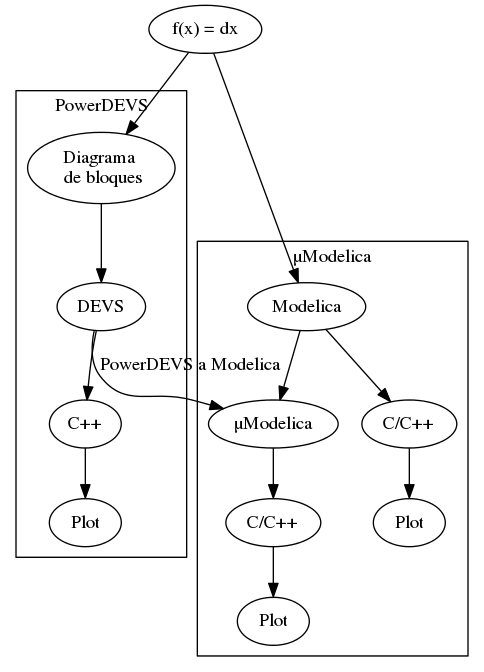
\includegraphics[width=0.75\linewidth]{esquema}
 \caption{Esquema de conversiones}
 \label{fig:esquema}
\end{figure}

En la figura \ref{fig:esquema}, se muestran los dos principales estrategias (PowerDEVS y Modelica) para realizar una simulación. En el caso de PowerDEVS, el primer paso es convertir el sistema en diagramas de bloques, luego en DEVS, en PowerDEVSe el cual puede automáticamente convertirlo en C++ y luego obtener los resultados ejecutando este modelo. 

Desde la perspectiva de Modelica (o $\mu$-Modelica), debemos pasar el sistema a Modelica (o $\mu$-Modelica) y luego el compilador se encargara de generar código (usualmente C o C++) capaz de correr la simulación y obtener resultados.

El actual trabajo está representado por la flecha que sale de PowerDEVS hacia $\mu$modelica, permitiendo especificar la simulación en diagramas de bloques y ejecutar la simulación en el QSS-Solver, en el lenguaje $\mu$modelica.

\section{Organización del presente trabajo}

\section{Motivación y Objetivos}
PowerDEVS\cite{BK11} es una herramienta de simulación de sistemas híbridos, basado en el formalismo DEVS\cite{Zeigler:2000:TMS:580780}, con una interfaz gráfica orientada a bloques, donde los bloques pueden ser conectados entre si, modificado sus parámetros, además permite conectarse con el entorno Scilab para poder utilizar expresiones y herramientas de cálculo provistas por este entorno.

La resolución de ecuaciones diferenciales ordinarias, requiere el uso de métodos de integración numérica. Todos los algoritmos tradicionales de integración se basan en la discretización de la variable independiente (que generalmente representa el tiempo).

Las rutinas que implementan estos algoritmos, se denominan solvers y existen gran variedad de implementaciones de los mismos en diferentes lenguajes de programación. Los Métodos de Integración Numérica QSS (Quantized State System), a diferencia de los métodos de integración tradicionales, realizan la discretización sobre las variables de estado. En consecuencia, convierten los sistemas continuos en sistemas de eventos discretos, y tienen grandes ventajas para simular sistemas con discontinuidades.

Si bien PowerDEVS, implementa la totalidad de los algoritmos de QSS, resultan ineficientes, dado que malgastan gran parte de la carga computacional en la transmisión de eventos entre submodelos.

Para solventar este hecho se desarrollo una familia de QSS stand-solver, el cual requiere un modelo descripto en lenguaje C el cual contiene las ecuaciones diferenciales, las funciones de cruce de cero así como la información estructural requerida por los algoritmos QSS. Estos solvers obtienen una mejora de rendimiento de hasta un orden de magnitud comparado con otras implementaciones DEVS.

Sobre este se desarrollo una herramienta la cual genera a partir de un modelo $\mu$-Modedelica \cite{Ber12} (un subconjunto del lenguaje Modelica) el modelo requerido para el QSS solver.

Con el objetivo de utilizar los mejoras de velocidad y mantener un entorno amigable con el usuario, se creo una herramienta capas de convertir un modelo PowerDEVS en un modelo $\mu$modelica.


\section{Trabajo relacionado}
En \cite{Ber12} se describe una extensión del Compilador OpenModelica el cual traslada modelos regulares Modelica a $\mu$modelica. 
ModelicaDEVS \cite{Beltrame06quantisedstate} es una librería Dymola que permite describir simulaciones DEVS en el Modelica, más específicamente en el entorno Dymola.
M/CD++ \cite{conf/mascots/DAbreuW05} es una herramienta para convertir simulaciones en un subconjunto de Modelica, a simulaciones DEVS.
DESlib \cite{Sanz09paralleldevs} es una librería para la descripción de modelos Parallel DEVS en Modelica.


\section{Alcance}
DEVS\cite{Zeigler:2000:TMS:580780}, Discrete Event System Specification (Especificación de Sistemas de Eventos Discretos), es un formalismo modular y jerárquico para modelar y analizar sistemas que pueden ser de eventos de tiempo discreto mediante tablas de transición, y con estados continuos que pueden ser descriptos por ecuaciones diferenciales.
En el formalismo clásico DEVS, los modelos atómicos capturan el comportamiento del sistema, mientras los modelos Acoplados describen la estructura del mismo.
En particular los modelos atómicos en PowerDEVS son descriptos en clases C++, mientras que la estructura se encuentra definida en archivos pds y pdm.
Modelica es un lenguaje de modelado, orientado a objetos, declarativo, para el modelado orientado a componentes de sistemas complejos.
Para poder realizar nuestro objetivo es necesario primero contar con un modelo en modelica\cite{Fritzson02modelica--} para cada atómico PowerDEVS\cite{BK11} que deseemos convertir. 

De esto se desprenden las siguientes limitaciones importantes:
\begin{itemize}
	\item La semántica de los modelos convertidos depende de los modelos equivalentes a los DEVS atómicos 
	\item Solamente podemos convertir modelos cuyos componentes atómicos hayan sido convertidos a $\mu$modelica.
\end{itemize}


